\chapter{理論}
\section{AIを用いた楽曲作成}
\subsection{MIDI}
AIによる曲制作では主にMIDIファイルの音楽データを使用する.MIDI ファイルには実際の音ではなく音楽の演奏情報(音の高さや長さなど)である.
本研究で用いるAIはこのMIDIファイルの情報を元に学習をする.また入出力の際もこの規格を用いる.
\subsection{Magenta}
本研究ではMagenta[1]を使用する.これは音楽などをTensorFlowを使って機械学習するライブラリであり,Google BrainがGitHab上に公開している.
Magentaではまず学習させたい音楽のMIDIデータをNoteSequence(magentaが扱うファイル形式)とよばれるデータフォーマットに変更する.それを学習用データセットと評価用データセットに変換したあと学習を行う.
このとき,一度に学習させるデータの数,学習を行う回数,ノード数を設定する.これをパッケージ化し,MIDIファイルとして新たに楽曲を生成するという流れである.これを図2.1に示す.
\begin{figure}[h]
    \begin{screen}
    \begin{center}
        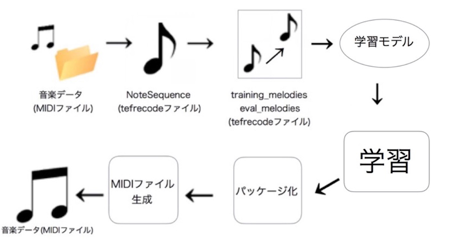
\includegraphics[scale=1.5, clip]{./img/magenta_usestep.png}
        \caption{magentaによるMIDI音楽データ生成までのプロセス}
        \label{fig:magentaによるMIDI音楽データ生成までのプロセス}
    \end{center}
    \end{screen}
\end{figure}\\
\newpage
\section{開発環境の構築}
本システムの開発環境を表\ref{tab:開発環境}に示す.
\begin{table}[h]
    \begin{center}
    \caption{開発環境}
    \label{tab:開発環境}
    \begin{tabular}{|c|p{30zw}|}
    \hline
    OS & OS X Yosemite\\
    \hline
    CPU & Intel Core i5\\
    \hline
    メモリ & 8GB\\
    \hline
    使用ライブラリ & TensorFlow ,magenta\\
    \hline
    \end{tabular}
    \end{center}
\end{table}\\
本システムは Macbook Pro を使用しOSは OS X Yosemite を使用した.
使用するライブラリとして,ニューラルネットワークを構築できるTensorflowを利用した.